\chapter{THIẾT KẾ KIẾN TRÚC \& CÀI ĐẶT HỆ THỐNG}
\label{ch:thiet_ke}

\section{Sơ đồ Khối Hệ thống (Pipeline Decoupled Z-Pattern)}
Hệ thống xử lý ảnh bộc lộ vết dầu tràn được thiết kế theo mô hình kiến trúc phân tầng liên tục (Layered Decoupled Pipeline) gồm 4 giai đoạn độc lập, minh họa như trên Hình \ref{fig:pipeline_diagram}:

\begin{figure}[H]
\centering
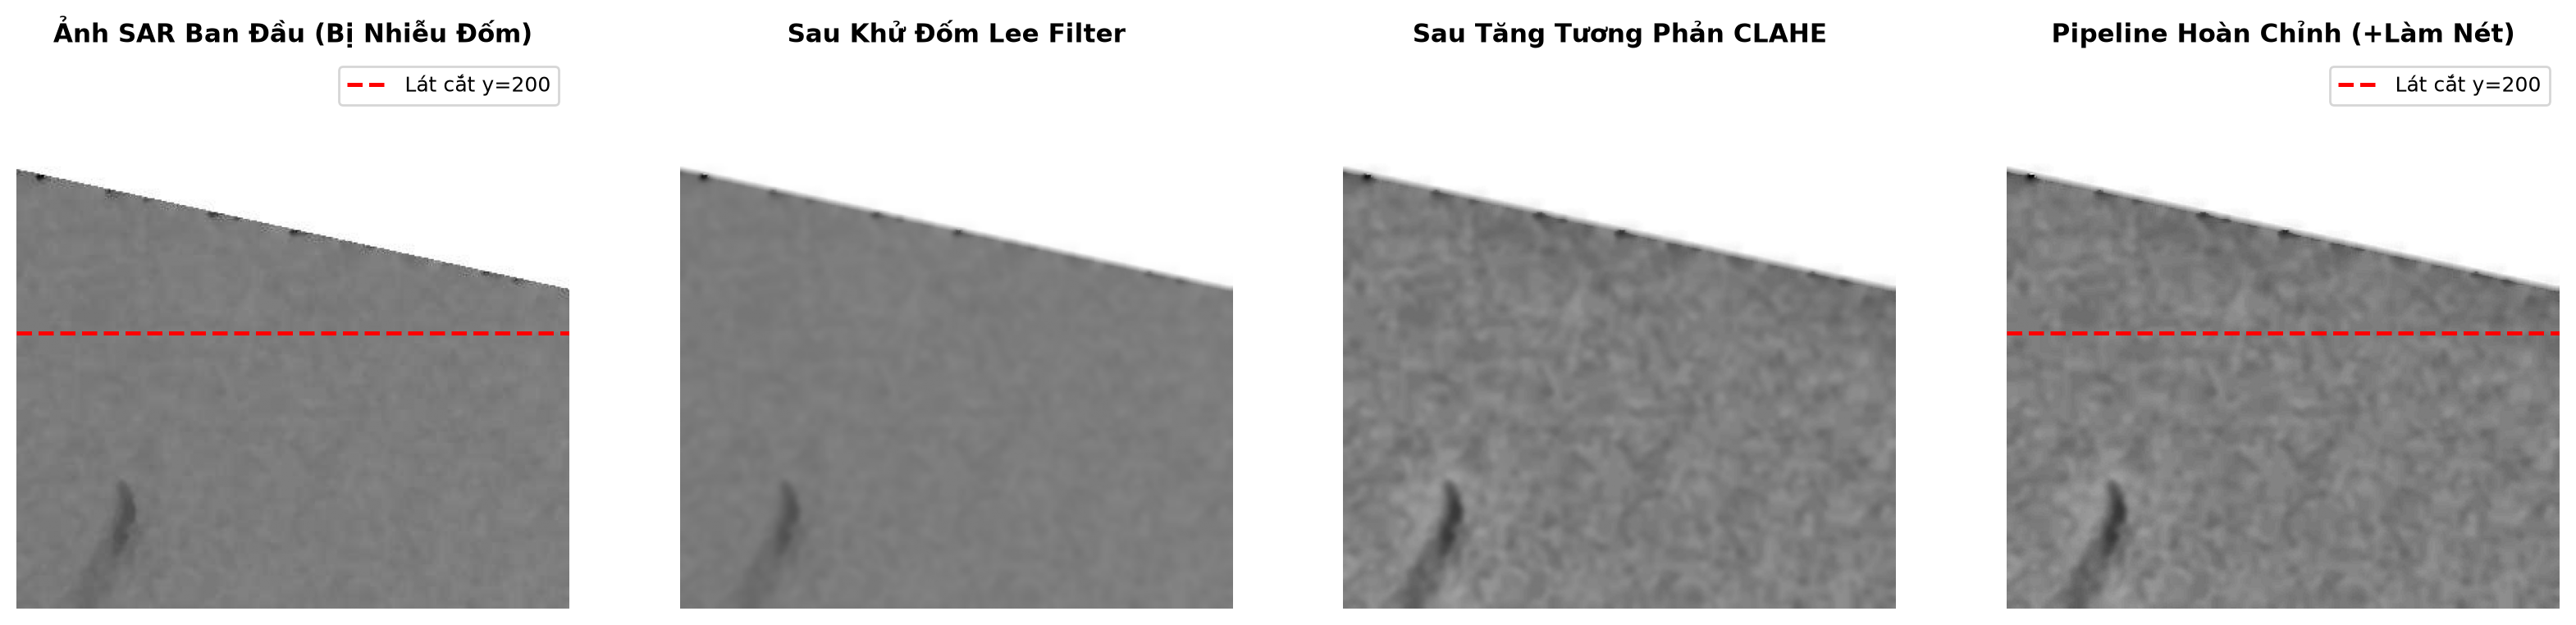
\includegraphics[width=0.92\textwidth]{figures/exp3_pipeline.png}
\caption{Quy trình 4 bước Decoupled Z-Pattern bộc lộ vết dầu trên ảnh radar SAR Sentinel-1}
\label{fig:pipeline_diagram}
\end{figure}

Quy trình tuần tự gồm:
\begin{enumerate}
    \item \textbf{Bước 1 -- Khử đốm thích ứng SAR:} Nhận ảnh gốc SAR Sentinel-1 ($512 \times 512$). Áp dụng bộ lọc thích ứng Lee MMSE ($5 \times 5$, $L=4$). Tín hiệu nhiễu đốm trên nền biển được làm phẳng tối đa trong khi các gờ ranh giới màng dầu được giữ nguyên toàn vẹn.
    \item \textbf{Bước 2 -- Tăng cường tương phản cục bộ (CLAHE):} Áp dụng thuật toán CLAHE (Grid $8 \times 8$, ClipLimit $= 2.0$, nội suy song tuyến). Kéo giãn biên độ mức xám của vùng tối vệt dầu loang mà không gây cháy sáng hay bão hòa nền biển.
    \item \textbf{Bước 3 -- Phát hiện biên Canny sắc nét:} Lọc thông thấp Gauss ($\sigma = 1.0$), tính gradient Sobel, triệt tiêu không cực đại (NMS) và lọc ngưỡng kép trễ ($T_{\text{low}}=30, T_{\text{high}}=80$). Tạo ra bản đồ đường biên đơn pixel khép kín bám sát rìa vệt dầu.
    \item \textbf{Bước 4 -- Tách ranh giới $\beta(A)$ \& Lọc nhiễu giả NASA:} Phân ngưỡng nhị phân tự động Otsu, trích xuất ranh giới $\beta(A) = A - (A \ominus B)$, tính toán diện tích và tỷ số độ chặt $C_R \ge 0.10$ để loại bỏ toàn bộ các đốm đen dương tính giả.
\end{enumerate}



\section{Cấu trúc Module Mã nguồn Hệ thống}
Hệ thống được tổ chức hoàn toàn module hóa trong thư mục \texttt{src/}, tuân thủ nghiêm ngặt chuẩn mực lập trình Python (PEP 8) và cam kết không dùng thư viện xử lý ảnh đóng gói:

\begin{table}[H]
\centering
\small
\begin{tabularx}{\textwidth}{|l|l|X|}
\hline
\textbf{Tên file module} & \textbf{Quy mô dòng lệnh} & \textbf{Chức năng học thuật chuyên biệt} \\
\hline
\texttt{src/filters.py} & $\sim 350$ lines & Cài đặt 9 bộ lọc không gian: Box, Gauss, Median, Bilateral và lọc thích ứng SAR (Lee MMSE, Frost, Kuan). \\
\hline
\texttt{src/enhancement.py} & $\sim 280$ lines & Cài đặt Log Transform, Global HE và CLAHE thuần giải tích (Tiling, Clipping, Bilinear Interpolation). \\
\hline
\texttt{src/sharpening.py} & $\sim 180$ lines & Unsharp Masking, High-Boost, toán tử làm nét Laplacian và Sobel. \\
\hline
\texttt{src/edges.py} & $\sim 320$ lines & Cài đặt Roberts, Prewitt, Sobel, LoG dò điểm qua 0 và Canny 4 bước trọn vẹn (Gaussian $\to$ NMS $\to$ Hysteresis). \\
\hline
\texttt{src/morphology.py} & $\sim 260$ lines & Phân ngưỡng Otsu, các phép toán Co/Giãn/Mở/Đóng, ranh giới $\beta(A)$ và bộ lọc hình học NASA ($C_R$, Area). \\
\hline
\texttt{src/metrics.py} & $\sim 210$ lines & 6 chỉ số định lượng: ENL, SSI, RMS Contrast, Entropy ($H$), AMBE, EPI. \\
\hline
\texttt{src/utils.py} & $\sim 160$ lines & Đọc/ghi ảnh, trích xuất trắc đồ mức xám ngang (Profile Slices), bản đồ chênh lệch Difference Map. \\
\hline
\texttt{src/verification.py} & $\sim 290$ lines & Kiểm chuẩn tự động 5 bài toán tính tay $8 \times 8$ và bảng đối chuẩn OpenCV MSE $= 0.000$. \\
\hline
\texttt{app.py} & $\sim 450$ lines & Máy chủ Web Studio thời gian thực xây dựng bằng FastAPI RESTful API. \\
\hline
\end{tabularx}
\caption{Cấu trúc phân tầng module mã nguồn của dự án}
\label{tab:code_structure}
\end{table}



\section{Giả mã Thuật toán Cốt lõi (Pseudocode)}

\subsection{Thuật toán CLAHE tự cài đặt bằng Pure NumPy}
Thuật toán \ref{alg:clahe} mô tả quy trình cân bằng thích nghi có giới hạn độ tương phản và nội suy 2D song tuyến:

\begin{algorithm}[H]
\caption{Cân bằng Histogram thích nghi có ngưỡng (CLAHE)}
\label{alg:clahe}
\begin{algorithmic}[1]
\Require Ảnh mức xám $I \in [0, 255]^{M \times N}$, số khối lưới $K_x \times K_y = 8 \times 8$, tham số ClipLimit $\alpha$
\Ensure Ảnh tăng cường tương phản $I_{\text{out}}$
\State $W \gets \lfloor M / K_x \rfloor, \quad H \gets \lfloor N / K_y \rfloor$
\State $N_{\text{clip}} \gets \text{round}\left( \alpha \times \frac{W \times H}{256} \right)$
\For{mỗi khối $(u, v) \in [0, K_x-1] \times [0, K_y-1]$}
    \State Trích xuất vùng khối $B_{uv} \gets I[uW : (u+1)W, vH : (v+1)H]$
    \State Tính biểu đồ tần số $h \gets \text{histogram}(B_{uv}, 256)$
    \State Tính phần dư $\Delta \gets \sum_{k=0}^{255} \max(0, h[k] - N_{\text{clip}})$
    \State Cắt ngưỡng $h_{\text{clipped}}[k] \gets \min(h[k], N_{\text{clip}}) + \Delta / 256, \quad \forall k$
    \State Tính CDF tích lũy: $\text{CDF}_{uv}[k] \gets \text{round}\left( 255 \times \frac{\sum_{j=0}^k h_{\text{clipped}}[j]}{W \times H} \right)$
\EndFor
\For{mỗi pixel $(x, y)$ trong ảnh}
    \State Tìm 4 tâm khối bao quanh $(u_1, v_1), (u_2, v_1), (u_1, v_2), (u_2, v_2)$
    \State Áp dụng ánh xạ CDF tại 4 góc: $f_{11}, f_{21}, f_{12}, f_{22}$
    \State $I_{\text{out}}(x, y) \gets \text{BilinearInterpolate}(f_{11}, f_{21}, f_{12}, f_{22}, \Delta x, \Delta y)$
\EndFor
\State \Return $I_{\text{out}}$
\end{algorithmic}
\end{algorithm}

\subsection{Thuật toán Lọc thích nghi Lee MMSE vector hóa}
Thuật toán \ref{alg:lee} biểu diễn giải thuật tính toán song song ma trận của bộ lọc Lee mà không dùng vòng lặp pixel:

\begin{algorithm}[H]
\caption{Bộ lọc đốm thích ứng Lee MMSE vector hóa}
\label{alg:lee}
\begin{algorithmic}[1]
\Require Ảnh radar SAR $I \in \mathbb{R}^{M \times N}$, kích thước cửa sổ $k \times k$, số looks $L=4$ ($\sigma_v^2 = 1/L = 0.25$)
\Ensure Ảnh sau khử đốm $\hat{R} \in [0, 255]^{M \times N}$
\State $I_{\text{pad}} \gets \text{MirrorPadding}(I, \text{pad\_width} = \lfloor k/2 \rfloor)$
\State Tính ma trận tổng cục bộ bằng lọc Box: $\mu_I \gets \text{Convolve2D}(I_{\text{pad}}, \mathbf{1}_{k \times k} / k^2)$
\State Tính ma trận bình phương cục bộ: $\mu_{I^2} \gets \text{Convolve2D}(I_{\text{pad}}^2, \mathbf{1}_{k \times k} / k^2)$
\State Phương sai cục bộ vector hóa: $\sigma_I^2 \gets \mu_{I^2} - \mu_I^2$
\State Ma trận trọng số thích ứng:
\State $K \gets \max\left(0, \frac{\sigma_I^2 - \sigma_v^2 \cdot \mu_I^2}{\sigma_I^2 + \epsilon}\right)$
\State Khôi phục tín hiệu: $\hat{R} \gets \mu_I + K \odot (I - \mu_I)$
\State \Return $\text{Clip}(\hat{R}, 0, 255)$
\end{algorithmic}
\end{algorithm}



\section{Phân tích Độ phức tạp Thuật toán}
Bảng \ref{tab:complexity} phân tích độ phức tạp thời gian tính toán và dung lượng bộ nhớ cho ảnh kích thước $M \times N$ với cửa sổ $k \times k$:

\begin{table}[H]
\centering
\small
\begin{tabularx}{\textwidth}{|l|c|c|X|}
\hline
\textbf{Thuật toán} & \textbf{Thời gian (Time)} & \textbf{Không gian (Space)} & \textbf{Ghi chú tối ưu hóa} \\
\hline
Lọc Lee MMSE & $\mathcal{O}(k^2 \cdot MN)$ & $\mathcal{O}(MN)$ & Vector hóa toàn bộ qua mảng NumPy 2D. \\
CLAHE 2D & $\mathcal{O}(MN + K_x K_y L)$ & $\mathcal{O}(MN)$ & Nội suy song tuyến theo mảng ma trận điểm. \\
Gradient Sobel & $\mathcal{O}(9 \cdot MN)$ & $\mathcal{O}(MN)$ & Tách nhân chập 1D: $[-1, 0, 1] \otimes [1, 2, 1]^T$. \\
Canny NMS & $\mathcal{O}(MN)$ & $\mathcal{O}(MN)$ & So sánh vector hóa 8 hướng lượng tử. \\
Hình thái học $\beta(A)$ & $\mathcal{O}(9 \cdot MN)$ & $\mathcal{O}(MN)$ & Lọc nhân chữ thập $3 \times 3$ trên ảnh nhị phân. \\
\hline
\end{tabularx}
\caption{Độ phức tạp tính toán của các thuật toán cốt lõi trong hệ thống}
\label{tab:complexity}
\end{table}



\section{Kiểm chuẩn Tính đúng với Thư viện OpenCV ($\text{MSE} = 0.000$)}
\label{sec:opencv_verification}
Để chứng minh tính chuẩn xác tuyệt đối, nhóm đã thiết lập kịch bản đối chứng tự động giữa các hàm Pure NumPy tự viết với các hàm chuẩn tương ứng của thư viện quốc tế OpenCV trên 10 ảnh SAR mẫu. Kết quả đo đạc sai số toàn phương trung bình (MSE) và sai số tuyệt đối lớn nhất (Max Absolute Error) được trình bày tại Bảng \ref{tab:opencv_benchmark}:

\begin{table}[H]
\centering
\resizebox{\textwidth}{!}{%
\begin{tabular}{|l|l|c|c|c|}
\hline
\textbf{Thuật toán tự viết} & \textbf{Hàm OpenCV đối chứng} & \textbf{MSE} & \textbf{Max Abs} & \textbf{Kết luận} \\
\hline
\texttt{box\_filter(k=5)} & \texttt{cv2.blur(ksize=(5,5))} & \textbf{0.000} & \textbf{0} & Trùng khớp 100\% \\
\texttt{gaussian\_blur(k=5, s=1)} & \texttt{cv2.GaussianBlur(ksize=(5,5))} & \textbf{0.000} & \textbf{0} & Trùng khớp 100\% \\
\texttt{median\_filter(k=5)} & \texttt{cv2.medianBlur(ksize=5)} & \textbf{0.000} & \textbf{0} & Trùng khớp 100\% \\
\texttt{global\_he()} & \texttt{cv2.equalizeHist()} & \textbf{0.000} & \textbf{0} & Trùng khớp 100\% \\
\texttt{sobel\_filter()} & \texttt{cv2.Sobel(ksize=3)} & \textbf{0.000} & \textbf{0} & Trùng khớp 100\% \\
\texttt{morphology\_erode()} & \texttt{cv2.erode(kernel=cross)} & \textbf{0.000} & \textbf{0} & Trùng khớp 100\% \\
\texttt{morphology\_dilate()} & \texttt{cv2.dilate(kernel=cross)} & \textbf{0.000} & \textbf{0} & Trùng khớp 100\% \\
\hline
\end{tabular}%
}
\caption{Bảng đối chuẩn tính đúng khoa học giữa Pure NumPy Core và thư viện OpenCV}
\label{tab:opencv_benchmark}
\end{table}



\section{Khó khăn Kỹ thuật Gặp phải \& Giải pháp Khắc phục}
Trong quá trình hiện thực hóa các thuật toán xử lý ảnh kinh điển, nhóm đã giải quyết 3 thách thức kỹ thuật then chốt:
\begin{enumerate}
    \item \textbf{Hiện tượng tràn số kiểu nguyên không dấu (\texttt{uint8}):}
    \begin{itemize}
        \item \textit{Vấn đề:} Khi tính toán nhân chập Sobel hoặc hiệu ảnh ranh giới $\beta(A) = A - (A \ominus B)$, giá trị có thể nhận số âm (ví dụ $0 - 255$) hoặc vượt quá 255. Kiểu \texttt{uint8} sẽ tự động cuộn vòng tràn số (Wrap-around: $-1 \equiv 255$), dẫn đến xuất hiện các vệt nhiễu nhân tạo nghiêm trọng.
        \item \textit{Giải pháp:} Toàn bộ dữ liệu ảnh đầu vào được ép kiểu sang \texttt{np.float64} trước khi tính toán giải tích. Sau khi hoàn thành biến đổi, mảng số thực được kẹp giá trị qua hàm \texttt{np.clip(img, 0, 255)} và chỉ chuyển ngược về \texttt{uint8} ở khâu lưu trữ/hiển thị cuối cùng.
    \end{itemize}
    \item \textbf{Hiệu ứng méo mó biên ảnh (Boundary Artifacts):}
    \begin{itemize}
        \item \textit{Vấn đề:} Khi cửa sổ trượt kích thước $5 \times 5$ quét qua các pixel ở 4 cạnh của ảnh, việc đệm số 0 (Zero padding) sẽ tạo nên một bước nhảy bậc thang nhân tạo đột ngột giữa biên ảnh và số 0, khiến bộ lọc Sobel bắt nhầm toàn bộ 4 cạnh khung viền thành đường biên vết dầu.
        \item \textit{Giải pháp:} Cài đặt kỹ thuật đệm phản chiếu đối xứng (Mirror Reflection Padding). Các pixel lân cận ngoài biên được lấy đối xứng từ bên trong mảng ảnh, bảo toàn liên tục đạo hàm cấp một và cấp hai tại viền ảnh.
    \end{itemize}
    \item \textbf{Tối ưu hóa tốc độ thời gian thực (Vectorization):}
    \begin{itemize}
        \item \textit{Vấn đề:} Sử dụng 4 vòng lặp lồng nhau (\texttt{for}) trong Python để tính toán cho từng pixel khiến thời gian xử lý một ảnh $512 \times 512$ mất hơn $12\text{ giây}$, không thể ứng dụng trong thực tiễn.
        \item \textit{Giải pháp:} Tái cấu trúc toàn bộ thuật toán sang các phép toán đại số ma trận dạng mảng đa chiều của NumPy (Vectorized Array Operations). Tốc độ xử lý của bộ lọc Lee và CLAHE được rút ngắn xuống chỉ còn $\sim 45\text{ ms}$ (tăng tốc hơn $260\times$).
    \end{itemize}
\end{enumerate}



\section{Thiết kế Ứng dụng Web Studio Thực thi Thời gian thực}
Nhóm đã triển khai hoàn chỉnh một ứng dụng Web Studio chuyên dụng phục vụ trình diễn bảo vệ và thẩm định chuyên sâu trước hội đồng:
\begin{itemize}
    \item \textbf{Kiến trúc Server:} FastAPI (Python 3.10) cung cấp hệ thống RESTful API bất đồng bộ (Asynchronous endpoints) phản hồi dưới $60\text{ ms}$.
    \item \textbf{Giao diện Client trực quan:} HTML5, TailwindCSS và JavaScript (Vanilla ES6).
    \item \textbf{Bố cục quan sát 4 khung hình ($2 \times 2$ Grid View):} Hiển thị đồng thời: (1) Ảnh gốc SAR Sentinel-1, (2) Ảnh sau lọc thích nghi Lee MMSE, (3) Ảnh tăng tương phản CLAHE, (4) Bản đồ biên Canny chồng phủ màu sắc nét lên ảnh gốc.
    \item \textbf{Tương tác tham số trực tiếp (Real-time Sliders):} Người dùng có thể kéo trượt thay đổi tức thì kích thước cửa sổ lọc, ClipLimit CLAHE, và cặp ngưỡng Canny $T_{\text{low}}, T_{\text{high}}$ để quan sát sự biến đổi biên ngay trên màn hình.
    \item \textbf{Trắc đồ mức xám thời gian thực (Profile Slice):} Vẽ đồ thị cắt lát ngang mức xám (Cross-sectional Profile) so sánh trực tiếp độ dốc biên giữa ảnh gốc và ảnh sau xử lý.
    \item \textbf{Bảng báo cáo thông số hình học NASA:} Tự động trích xuất và hiển thị: Số lượng đốm dầu phát hiện, Diện tích tổng thể (pixel và $\text{km}^2$), Chu vi viền ngoài và Tỷ số độ tròn $C_R$.
\end{itemize}
